\subsection{NUNAV Navigation}

Der NUNAV-Routingalgorithmus ist bei Graphmasters in verschiedene Produkte integriert. Eines der Produkte ist \textit{NUNAV Navigation}. Dies ist eine frei verfügbare Navigationssoftware für Smartphones, deren Zielgruppe Endanwender sind, welche eine geführte Navigation nutzen wollen (mehr siehe \autoref{sec:06_model_evaluation:personas}). Mithilfe dieser können sich Privatanwender wie von bekannten Navigationslösungen gewohnt, zu beliebigen Zielorten navigieren lassen. Darüber hinaus haben Nutzer die Möglichkeit direkt nach Veranstaltungen und von NUNAV verwalteten Orten zu suchen. Dabei können Veranstalter NUNAV als individuelles Parkleitsystem einsetzen. Navigieren Nutzer mit \textit{NUNAV Navigation} zu einem verwalteten Suchergebnis, werden sie auf einen freien Parkplatz geführt. Dabei kann auch zwischen verschiedenen Rollen unterschieden werden. So können Aussteller von Messen zum Beispiel direkt zum richtigen Eingang navigiert werden, statt auf einen Besucherparkplatz.

Für diese Arbeit dient die bestehende App \textit{NUNAV Navigation} als Grundlage für die Integration von Erklärungen und ist somit das \textit{System}, für das die Erklärbarkeit im Kontext der Anwendung des vorgestellten Leitfadens verbessert werden soll.

\subsubsection{Technischer Überblick}

Im Allgemeinen setzt die Graphmasters GmbH auf eine \textit{Micro-Service}-Infrastruktur. Das bedeutet, die einzelnen Teilsysteme der NUNAV-Technologie sind stark gekapselt und werden unabhängig voneinander bei mehreren Cloud-Infrastruktur-Anbietern betrieben. So ist nicht nur eine unabhängige Entwicklung möglich, sondern auch die Skalierung einzelner Systeme ist einfach und kostengünstig umsetzbar. Clients für die Services sind entweder mobile Anwendungen für Smartphones oder Webanwendungen.

\begin{figure}[htb!]
    \centering
    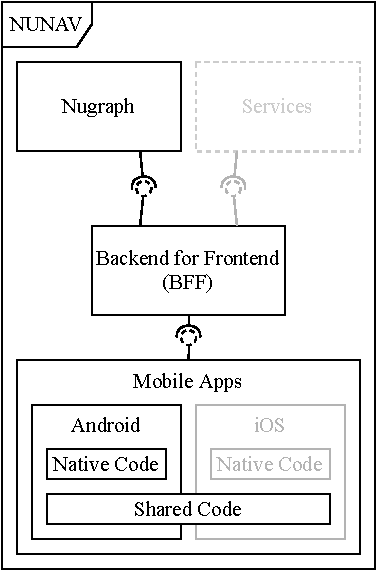
\includegraphics[width=\textwidth]{contents/06_model_evaluation/01_integration/res/nunav_architecture.pdf}
    \caption{Ausschnitt aus der NUNAV Software Architektur (UML-Komponenten-Diagramm)}
    \label{fig:nunav_software_architecture}
\end{figure}

\autoref{fig:nunav_software_architecture} stellt abstrakt alle für diese Arbeit relevanten Services der Infrastruktur dar. Wichtig ist dabei zum einen der Routingalgorithmus an sich (\textit{Nugraph}), welcher die Daten für die Navigation bereitstellt. Zum anderen ist die mobile Anwendung von \textit{NUNAV Navigation} relevant, da dort Erklärungen integriert werden sollen. Außerdem gibt es für jede Client-Anwendung einen sogenannten \textit{Backend for Frontend} (BFF). Für die mobilen Anwendungen ist dies der \textit{Mobile BFF}. Dieser stellt die einzige Kommunikationsschnittstelle der Clients mit allen anderen Services der Infrastruktur dar. In der Regel wird die Kommunikation zwischen den Services bzw. Clients und dem BFF über REST
\footnote{\textit{Representational State Transfer} ist ein Paradigma zum Austausch von Daten über das HTTP-Protokoll.}
-Schnittstellen mit JSON
\footnote{\textit{JavaScript Object Notation} ist ein Datenformat, welches vor allem für Maschine-zu-Maschine-Kommunikation eingesetzt wird und Programmiersprachen unabhängig ist.}
als Übertragungsformat abgewickelt. 

\paragraph{Nugraph} \textit{Nugraph} ist der Gesamtbegriff in der Architektur für die Services, welche zum Routingalgorithmus gehören. Dieser berechnet auf der Basis eines prädiktiven Verkehrsmodells die individuell schnellste Route zwischen zwei Punkten. Dabei wird anhand von ca. 1,5 Millionen Verkehrsmessungen
 (z.B. \textit{Floating Car Data}\footnote{\textit{Floating Car Data} (FCD) sind mit Zeitstempeln versehene Geolokalisierungs- und Geschwindigkeitsdaten, die direkt von fahrenden Fahrzeugen erfasst werden.})
 in der Minute der Verkehr auf der Route mithilfe von künstlicher Intelligenz vorausgesagt. Alle Daten die zur Navigation (z.b. Verlauf und Geschwindigkeit auf der Route) benötigt werden kommen von diesem Teilsystem.

\paragraph{Backend for Frontend} Der in \autoref{fig:nunav_software_architecture} gezeigte \textit{Mobile-BFF} ist zum einen für die korrekte Weiterleitung von Anfragen an den richtigen Service zuständig. Darüber hinaus bereitet dieser auch Daten anderer Services für die Mobilen Apps auf oder konvertiert die verschiedenen Formate. Dabei werden zum Teil Daten mehrerer Services gebündelt oder neue Daten berechnet. 

\paragraph{Mobile Apps} Die mobilen Anwendungen für Smartphones bereiten zum einen die Daten der \textit{Micro-Services} für die Nutzer auf und zeigen sie diesen an. Zum anderen verarbeiten diese lokal die vom BFF bereitgestellte Routen. Dabei berechnen die Applikationen die Position auf der Route, zum Geben von Abbiege-Kommandos und Anzeigen des Routenverlaufs. Die \textit{Mobile Apps} werden für Android und iOS parallel in den jeweiligen vom Hersteller bereitgestellten Frameworks nativ entwickelt. Außerdem gibt es eine geteilte Code-Basis, welche Kotlin-Multiplatform\footnote{\textit{Kotlin-Multiplatform} ist eine Technologie zur Kompilierung von Kotlin-Code in Binärdaten für verschiedene Platformen und Prozessorarchitekturen.} als Technologie nutzt.

\bigskip

Die drei vorgestellten Systemteile können entweder Daten für Erklärungen liefern oder sind für die Auslieferung der Erklärungen an sich zuständig. Im Rahmen dieser Arbeit wurden dabei sowohl auf dem BFF, als auch in der Mobilanwendung für Android Änderungen vorgenommen. Außerdem wurden Änderungen von der Graphmasters GmbH in \textit{Nugraph} und einem weiteren Service vorgenommen, um benötigte Daten für die entwickelten Erklärungen zur Verfügung zu stellen.